\documentclass[journal,10pt,onecolumn,compsoc]{IEEEtran} \usepackage[margin=1.0in]{geometry} \usepackage{pdfpages} 

%\usepackage{color}
\usepackage{geometry}
\usepackage{graphicx}
\usepackage{amsthm}
\usepackage{amssymb}
\usepackage{amsmath}
\usepackage{float}
\usepackage{balance}
\usepackage{enumitem}
\usepackage{pstricks, pst-node}
\usepackage{hyperref}
\usepackage{url}

\hypersetup{
  colorlinks = false,
  urlcolor = black,
  pdfkeywords = {CS461``Senior Software Engr Project''Design Document},
  pdftitle = {CS 461 Design Document},
  pdfsubject = {CS 461 Design Document},
  pdfpagemode = UseNone
}

\begin{document}
\begin{center}
  
  \textbf{}

  \vspace{2.5cm}
  \Huge{}
  \textbf Design Document
  \vspace{1.5cm}

 
  \LARGE
  CS461 - Senior Software Engr Project\\
  \vspace{0.25cm}
  Instructor: D. Kevin McGrath \\
  Instructor: Kirsten Winters \\
  \vspace{0.25cm}
  Fall 2018 \\
  \vspace{1cm}
  
  \large{Matthew Jansen, Bhavya Parikh, Davian Lukman, Eli Laudi, Ryan Sisco}\\
  \vfill
  November 26th, 2018\\
  \vspace{1cm}
  \vspace*{\fill}
   \begin{abstract}
      The purpose of this document to describe our design components and steps. The document includes a glossary, different technologies, and methodologies which will be made use of in the project. It also includes the reasoning and justifications behind our design choices made on the project. This will thus act as our road map  for our project over the year.
       \noindent 
   \end{abstract}
   \normalsize 
  \end{center}
\newpage
\tableofcontents
\newpage

\section{Overview}
    \subsection{Scope}
    The software depicted in this document expresses a web application used for converting data from CSV-file format to a 3D environment with an integrated time line. Our objective is to develop an application that supports client presentations and allows for better understanding of the relationships between large data sets.
    \subsection{Purpose}
    The purpose of this document is to analyze how DIVA is designed. To accomplish this, we will describe an overview of our web application, and provide technical details of the systems architecture and different functionality.  
    \subsection{Intended Audience}
    The intended audience for this project are the users who want to visualize their data preferably from the CSV data file in a 3D visual environment where they can alter the data points and relationship between multiple objects in a real time. 
    \subsection{Conformance}
    A web application conforms to this standard if it satisfies all of client mentioned/ required requirements.

\section{Definitions}
    \textit{DIVA: } Data Interactive Visualization Application; The name of the web application under development. \\
    \textit{CSV: } Comma Separated Value file; A delimited text file that uses a comma to separate values. A CSV file stores tabular data in plain text. Each line of the file is a data record. \\
    \textit{WebGL:} Web Graphics Library; Allows rendering using the graphics card on a JavaScript web application.\\
    \textit{HTML:} Hypertext Markup Language; The standard markup language for creating web pages and web applications. \\
    \textit {JavaScript: }JavaScript is a programming language commonly used in web development. \\
    \textit{CSS: }Cascading Style Sheets; A style sheet language used for describing the presentation of a document written in a markup language like HTML. \\
    \textit{JSON: }JavaScript Object Notation; An open-standard file format that uses human-readable text to transmit data objects consisting of attribute–value pairs and array data types\\
    \textit{IOC: }Indicator of Compromise; An indicator or identification which consist of IP address and hash value of compromise.\\
    \textit{SRS: }Software Requirements Specification.\\
    \textit{GIF: }Graphics Interchange Format; A GIF is a format which plays multiple frames in a loop without sound.\\
    \textit{PNG: }Portable Network Graphics is a raster graphics file format that supports lossless data compression\cite{PNG}.\\
    \textit{MP4: }MP4 is a file format created as a multimedia container format designed to store audiovisual data.\\
    \textit{MOV: } Apple Quicktime Movie file; A common multimedia container file format developed by Apple and compatible with both Macintosh and Windows platforms \cite{MOV}.\\
    \textit{UML: }Unified Modeling Language; A language in the field of software engineering, that is intended to provide a standard way to visualize the design of a system\cite{UML}.\\ 
    \textit{WebM: } Web Media library; A high-quality, open video format that is designed for the web \cite{WebM}.\\
    
\section{Conceptual Model for Software Design Descriptions}
    \subsection{Software Design in Context}
    For the user to use this software, they need to first make sure that they have a CSV data file. The CSV data file is a delimited text file that uses a comma to separate values. It stores tabular data in plain text. The user must have their data inputted and saved in the CSV file, where they have at the least three separate columns of data. By making use of the web application they the user will be able to upload the CSV file through an file explorer on the web application. The web application will give the user graph options after selecting the option the user must click on the submit button. After which the application will format parse the CSV file using JSON and then the JSON data using the WebGL rendering will create a three dimensional representation of the data given by the user in the CSV file. The flow of the software design can also be seen the following figure 1.
    \begin{figure}[H]
        \centering
         \caption{Software Design}
         
\includegraphics[width=\linewidth]{designDocFlowchartEdit.png}
        \label{fig:my_label}
    \end{figure}
    \subsection{Software Design Descriptions Within the Life Cycle}
    For this project we will be using the software development life cycle. It is the approach to software development under which requirements and solutions evolve through the collaborative effort of self-organizing and cross-functional teams and their customer and users. Thus our life cycle for our software using this methodology would be as follows:
    \begin{itemize}
    \item Step1 : Product Backlog Creation
    \item Step2 : Sprint Planning and Sprint Backlog Creation 
    \item Step3 : Working on the Sprint and Scrum meetings
    \item Step4 : Testing and Product Demonstration
    \item Step5 : Retrospective and Next Sprint Panning
    \end{itemize}
\section{Design Description Information Content}
    \subsection{Introduction}
    The following section will describe the general design of the DIVA web application. This section will include an identification and definition of this projects SDD, design stakeholders, and design concerns. Furthermore, this section will define selected design viewpoints, views, overlays, and our design rationale. 
    \subsection{SDD Identification}
        \subsubsection{Date of issue and status}
        The project is issued at September 2018 and the project status is ongoing. Expected to be finish at June 2019.
        \subsubsection{Scope}
        The software depicted in this document expresses a web application used for converting data from CSV-file format to a 3D environment with an integrated timeline. Our objective is to develop an application that supports client presentations and allows for better understanding of the relationships between large data sets.
        \subsubsection{Issuing Organization}
        McAfee is an American global computer security software company is the issuing organization that propose the project to our university, Oregon State University as medium to do software engineering project.
        \subsubsection{Authorship}
        The authorship of this document and project belongs to Matthew Jansen, Bhavya Parikh, Davian Lukman, Eli Laudi, and Ryan Sisco.
        \subsubsection{References}
        Professor:\\
        Kirsten Winters: wintersk@oregonstate.edu\\
        Kevin D. McGrath: dmcgrath@oregonstate.edu
        \subsubsection{Context}
        DIVA is the product that display a 3D data visualization in subject of interest; in this case, cyber-security data. DIVA can produced a data visualization  consisting of a map and a chart. The visualization will be taken from a CSV file and can be exported in another format.\\
        DIVA is prepared to help scientist better visualize their data in term of CSV file. The content of DIVA can be interacted as part of interactive object and relationship to the data. 
        \subsubsection{Language}
        The application will be written in a combination of JavaScript, HTML, and WebGL commands.
        \subsubsection{Summary}
        The purpose of this document is to analyze how DIVA is designed. To accomplish this, we will describe an overview of our web application, and provide technical details of the systems architecture and different functionality.  
        \subsubsection{Glossary}
        Parsing: process of analyzing a string of symbol.\\
        Structure: organize, management, and storage format to ensure efficient access or modification.\\
        Interactive: allow two flow information between the users and interface.\\
        Redux: Open source JavaScript library.
    \subsection{Design Stakeholders and Their Concerns}
    The stakeholder for this project is Christiaan Beek, Director of Threat Intelligence at McAfee Labs Intel Security. The project should be fast, easy to use, and produce a visually pleasing generation of the given data.
    \subsection{Design Views}
    The user and the developer of this application have a different views because each perspective reduces how each see the system. The view of the user consist of the choosing which file to be inputted, setting up graph options, and seeing the 3D visualization of data in which the user can interact with. By definition, the user cannot see any details that is going on inside the database or how the 3D visualization is made out of.\\
    On the other hand, the developer view of this application is a source code of HTML, and JavaScript as tools for this app. This does not include actual data that the user input, and connection with the users. Therefore, user's data will remain private.
    \subsection{Design Viewpoints}
    The viewpoint of this application is divided into two, which how the user see the application and how the developer see the application. The user describe the application from their perspective, including user usability, response time, data accuracy, rendering performance, and access to final product. While the developer describe the application quite different than the user, which is using HTML and JavaScript to make connection between data inputted and visualization data. 
    \subsection{Design Elements}
        \subsubsection{User Interface}
        The user interface will be constructed using React and Redux.  React is a JavaScript library for building high speed, often single page, web applications. Redux is a predictable state management container for JavaScript apps.
        The purpose of using both of these technologies is to make a user interface that is fast and can seamlessly integrate with the other portions of the application. Utilizing React, it is possible to include several third party libraries that will make the appearance of the web page cleaner without the overhead of writing our own CSS. Redux will be our main method for gathering the input from the user into one space. Doing so will allow the application to render a graph based on user input that has one source of truth. As a stretch goal, there is a possibility to create a back-end to serve up saved CSV files. Redux will allow the expansion into that area with very little changes to the code base.
        
        \subsubsection{CSV Processing}
        The CSV will be format parsed through JSON using JavaScript jQuery to form a better object structure that takes IOC as the parent, and other details as child. For example, the child in this project will consist of Date, Location type, and type of IOC.
        \begin{figure}[H]
            \centering
            \caption{JSON architecture sample}
            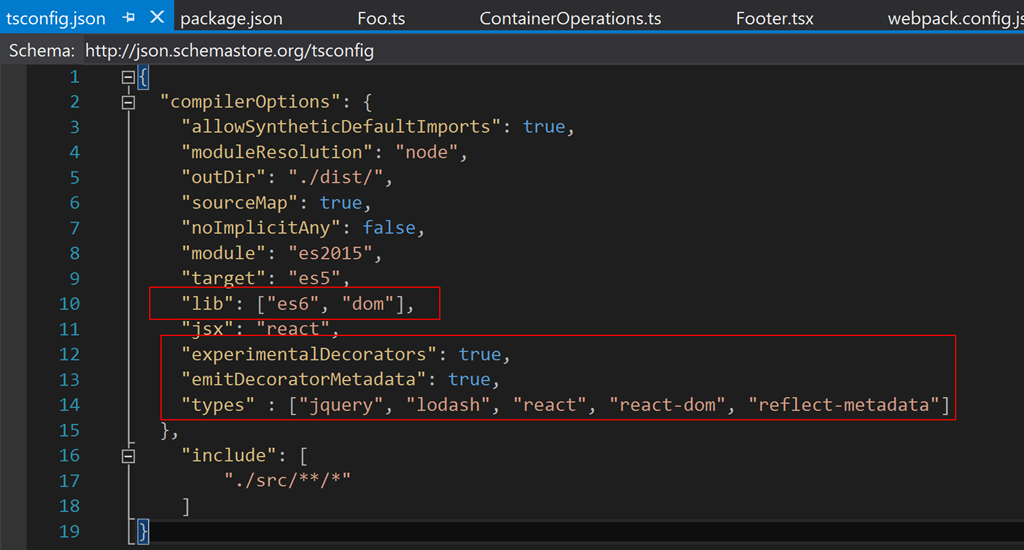
\includegraphics[width=\linewidth]{json.png}
        \end{figure}
        \subsubsection{WebGL}
        WebGL is a JavaScript library that gives the user 2D and 3D rendering capabilities. It is very flexible and allows the user to choose each element and how it is generated. It is well documented and is open source. This allows for a very complex design or the ability to use a very simple one. There are very complex and detailed graphics created with WebGL that involve a lot of time and creativity to build \cite{Jellyfish}.
        \begin{figure}[H]
            \centering
                \caption{WebGL Complicated Example}
                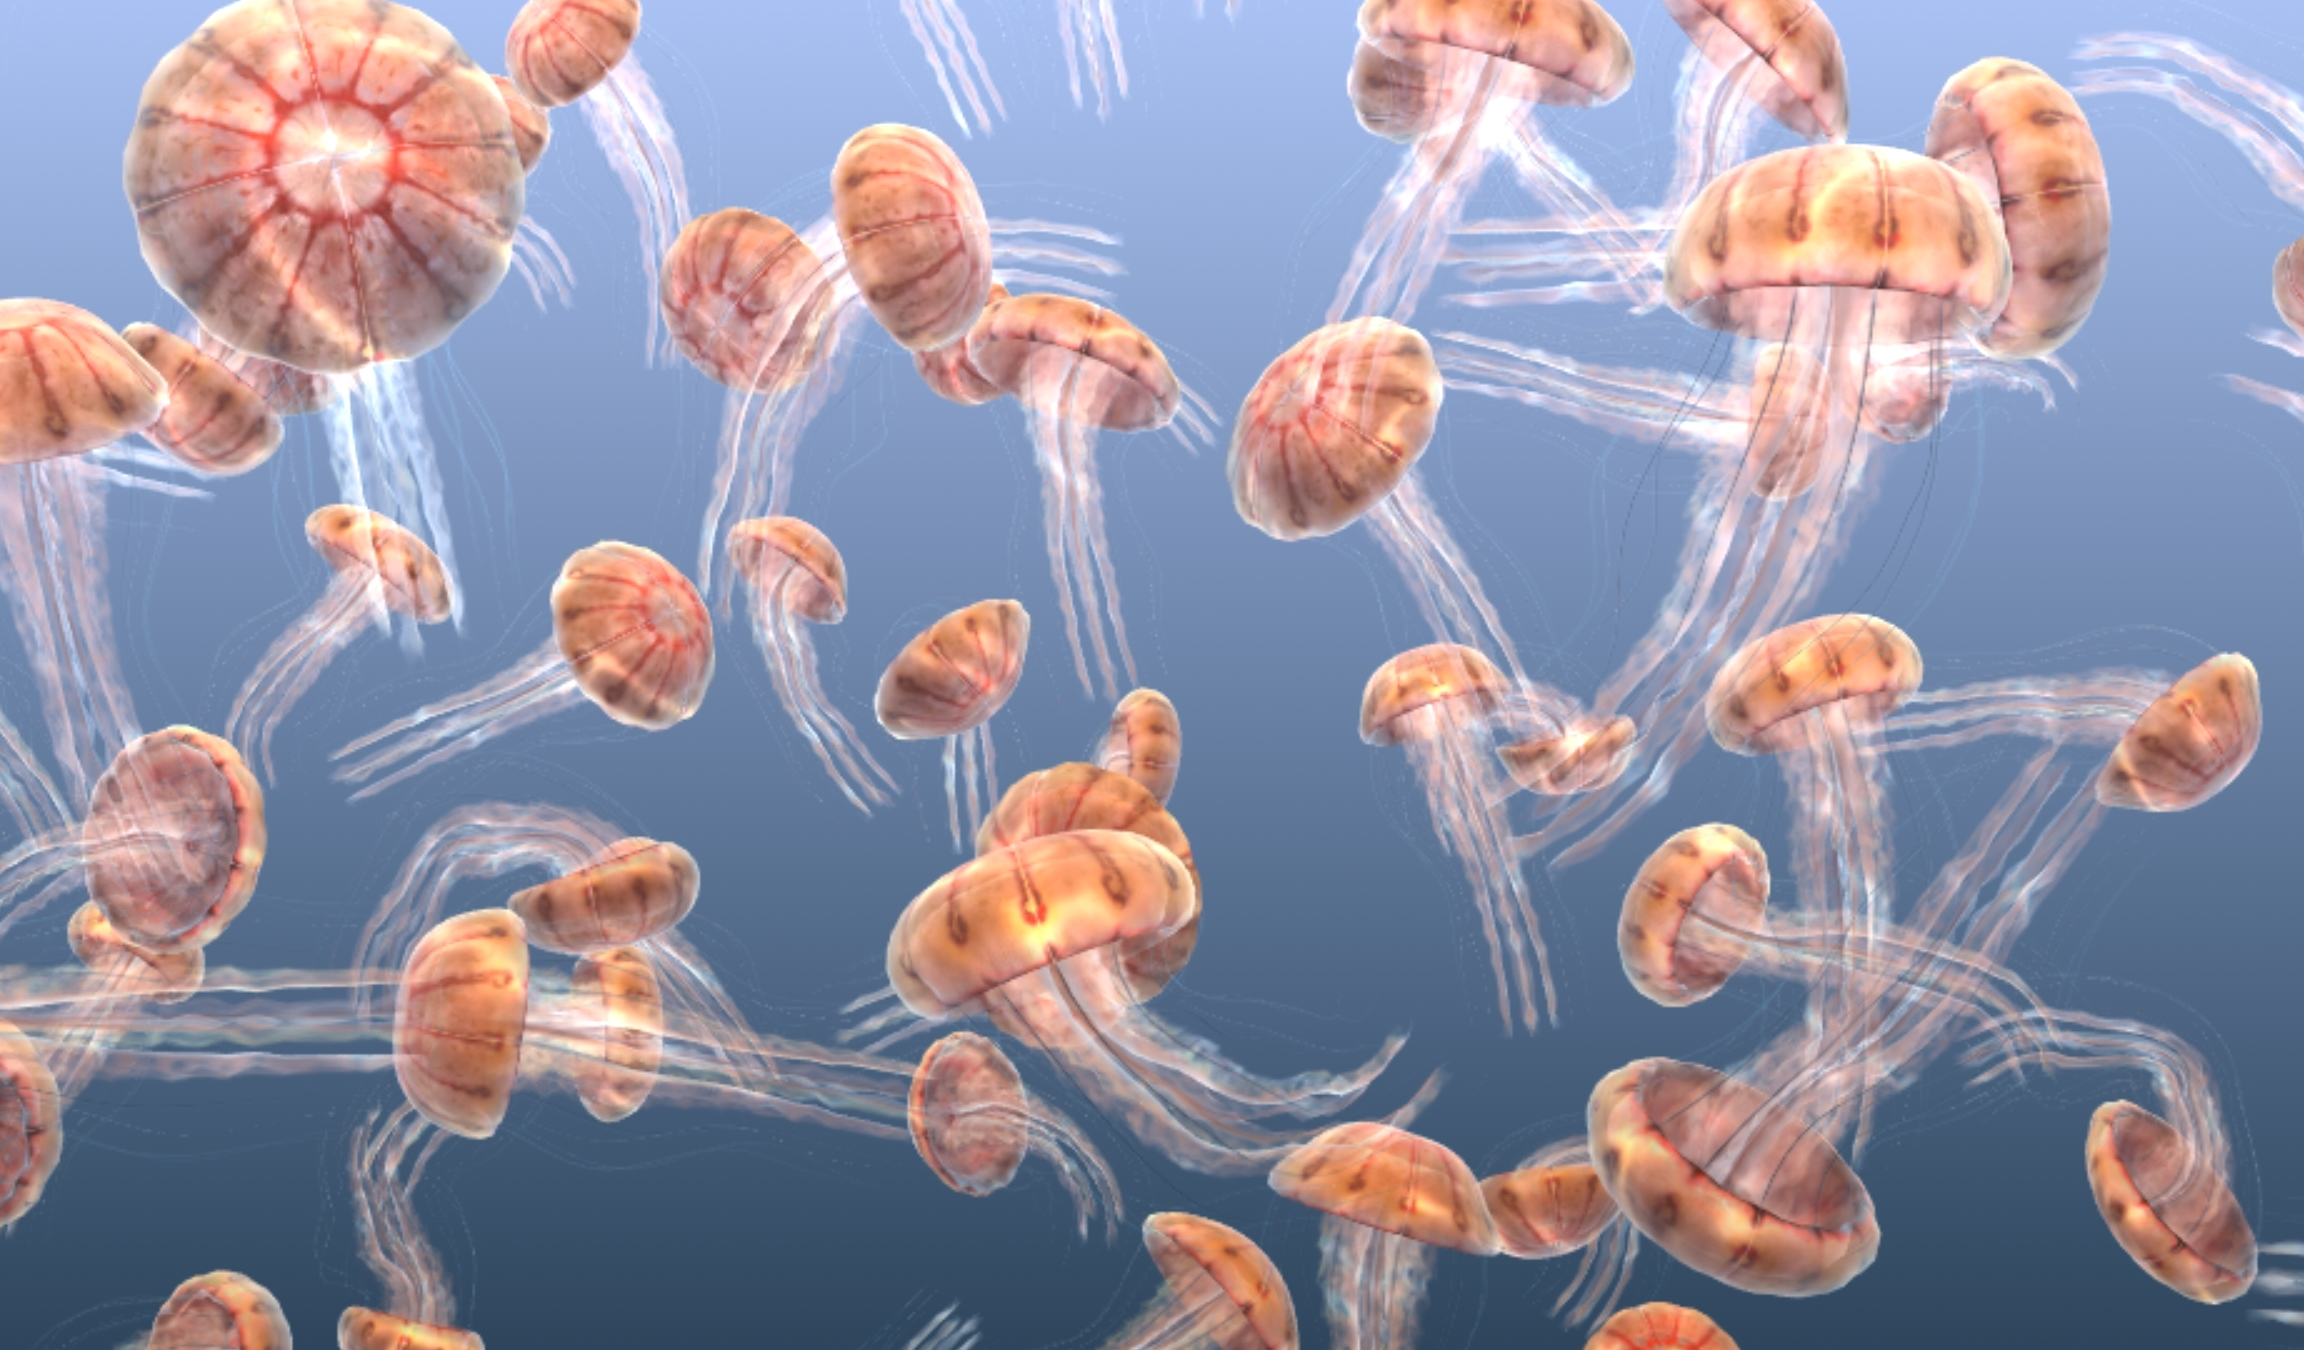
\includegraphics[width=\linewidth]{webgl_example_1.jpg}
        \end{figure}
        We plan on using this technology in conjunction with our CSV processing and user interface, to take data and populate a 3D render as well as a 2D graph. Both graphs should have the ability to be interacted with, including position and an animated time-line. Plotting points with WebGL is very easy to do, and there are several examples showing this. The points can be rearranged to fit any shape desired by the programmer, but if implemented correctly, the user should be able to specify any predefined shapes \cite{Plots}.
        \begin{figure}[H]
            \centering
                \caption{WebGL Plotting Points}
                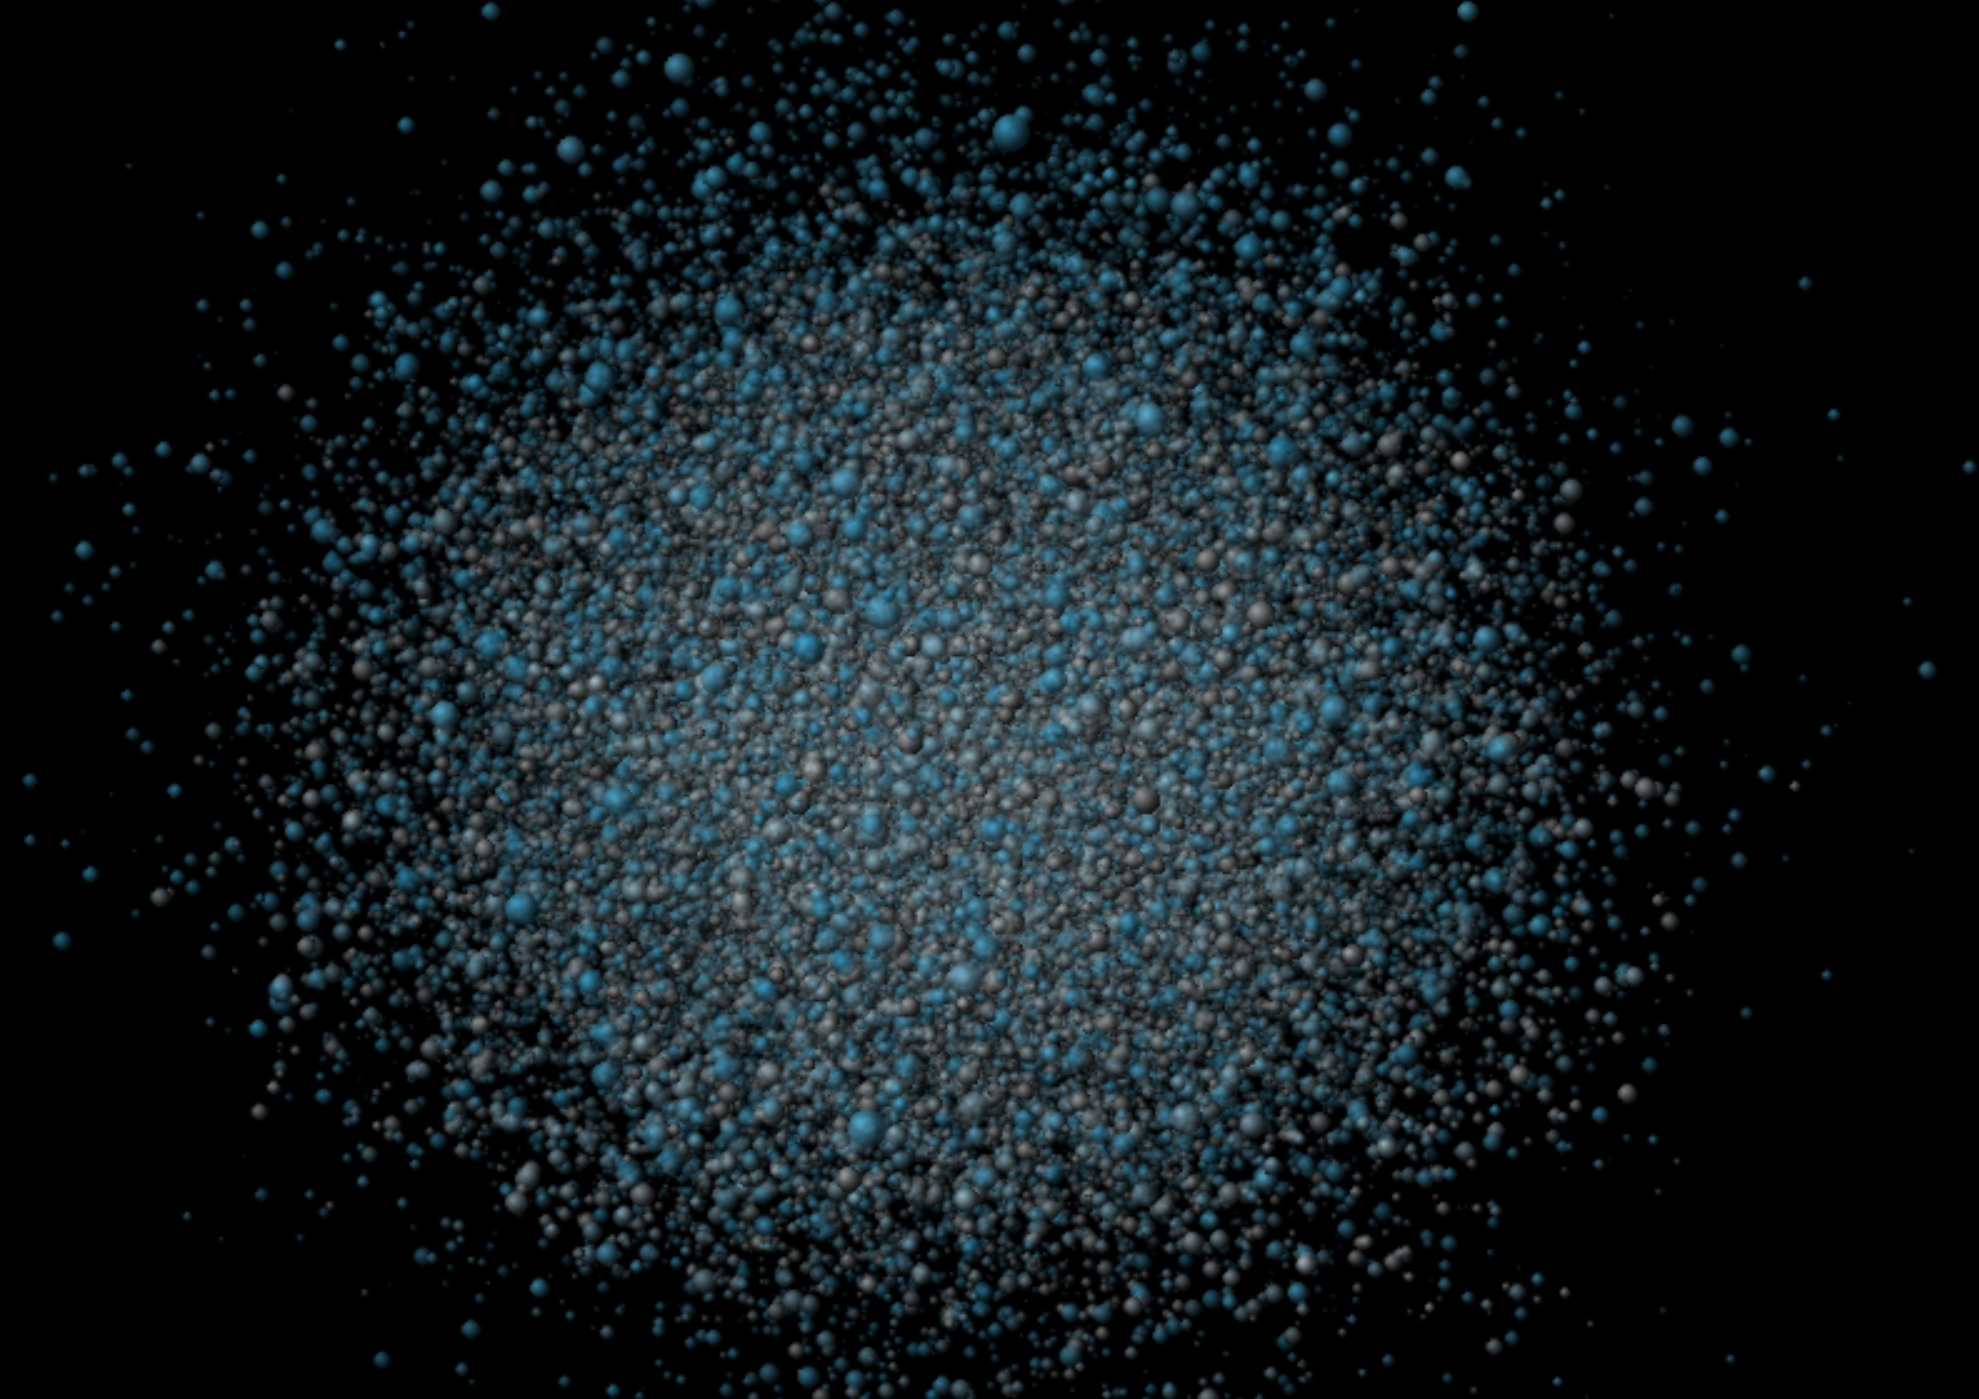
\includegraphics[width=\linewidth]{webgl_example_2.jpg}
        \end{figure}
        \subsubsection{Media Export}
        As one of the key features of this application is to show off the 3D graphical data, exporting the data in some form of picture, animation, or movie is quite important. In order to create these media, the application must have a way to record the current animation. There are a few JavaScript libraries that can greatly assist with this challenge. \\
        First, for exporting a simple image, is html2canvas \cite{html2canvas}. This library allows a user to screen shot a specific frame of a web browser, which in our case would be the window in which the 3D graph is being rendered. After the screen shot is taken, a simple download link will appear where the user can obtain the image.\\
        As capturing data in three space and being able to manipulate and view the data is a large facet of the project, the ability to capture multiple frames in a media export is very important. There are two different methods for this approach: a GIF or a MOV/MP4 file. GIFs can be created in a very similar way to single frame captures. Utilizing the third party library gif.js \cite{gif.js}, the application is able to capture multiple frames using the html2canvas method and compile them into a GIF. After compilation, a prompt for the download link can be provided to the user. In order to generate an MP4 file, there are two JavaScript libraries that will be used: whammy.js\cite{whammy.js} and ffmpegserver.js \cite{ffmpegserver.js}. These two libraries each manage a different section of the pipeline in the generation of an MP4 file. Whammy will continually take snapshots of the desired canvas area and compile them into a webm file type. After obtaining the webm file, ffmpegserver.js will spin up a node server that takes in canvas frames and generates an MP4 or MOV file from them. After all the frames are rendered in the desired file type, the file is made available to the user.
    \subsection{Design Overlay}
        \subsubsection{CSV input}
        1. loadFile, overlay to drag or load CSV file from local computer\\
        2. renderOption, overlay to define what kind of environment suitable for the visualization
        
        \subsubsection{Rendering}
        1. colorOverlay, an overlay to change the color for the chart\\
        2. editOverlay, an overlay that allow the user to edit the graph
        
        \subsubsection{Export}
        1. exportData, an overlay that has the options to printout the result as various format
        
    \subsection{Design Rationale}
    Based on the requirements, our rationale for going with our web application design is the freedom it gives the user. A web application can be served up over the internet allowing a user to access it even if they don't have the application on their machine. If a user wants to use the graph outside of the web app, they can export the graph as a different form of media (video or image) and insert it into a presentation.
    \subsection{Design Languages}
    The application will be written entirely in JavaScript with the exception being the parts of WebGL that need to be passed as c++ code. 

\section{Design Viewpoints}
    \subsection{Introduction}
    This section catalogs some of the design viewpoints that were relevant to the DIVA 3D  Visualization web application. Each design viewpoint will be associated with a name, relevant design concerns, and any appropriate design languages. 
    \subsection{Context Viewpoint}
    During the development of the DIVA web application, it is important to consider how the end users will be utilizing the program in a general sense. In other words, the DIVA web application should be viewed from a "black box" perspective so that the functionality most used by our end users will be given the appropriate attention.
        \subsubsection{Design Concerns}
        During the design phase of the DIVA web application, the development team recognized that the intended application users could span over different levels of computer software experience. Some end users could have years of computer programming experience or in using data visualization tools, while for other users, this could be their first run-in with using tools of this nature. To ensure that end users of all experience levels are able to use the DIVA web application, special care will be given towards the development of any functionality which require user interaction, such that the instructions regarding the use of the application will be clear and concise. 
        \subsubsection{Design Elements}
        \textit{Design Entities: } The actors that will be interacting with the DIVA web application include end users and stakeholders of the system. Other external systems which might interact with the DIVA web application can include systems which hold logging and exporting capabilities, specifically exporting CSV file types which can act as input to the application. \newline
        \newline \textit{Design Relationships: } Including the actors and external systems defined in the \textit{design elements} sub-section, we expect the 3D environment output of the DIVA web application to have direct relation to the CSV file input given by any actor. The relationship the input data (CSV file) and the output data (3D environment) hold is defined by the properties of the input data, and how it is digested by the WebGL rendering methods. \newline
        \newline \textit{Design Constraints: } The qualities of the DIVA web application include processing data from a CSV file format into a 3D environment, using WebGL, with rendered data points and relationships, as well as a timeline functionality. The 3D environment will first be rendered to the user's web browser, however the user will also have the ability to export the rendered environment to a picture (PNG), animation (GIF), or movie (MOV, MP4) file format.
        \subsubsection{Example Languages}
        UML use cases will be best suited for the design process of the DIVA web application. The image below depicts the users interaction with the system, with the interactions placed in the chronological order of the users actions. 
            \begin{figure}[H]
                \centering
                    \caption{UML Use Case Diagram for DIVA Web Application}
                    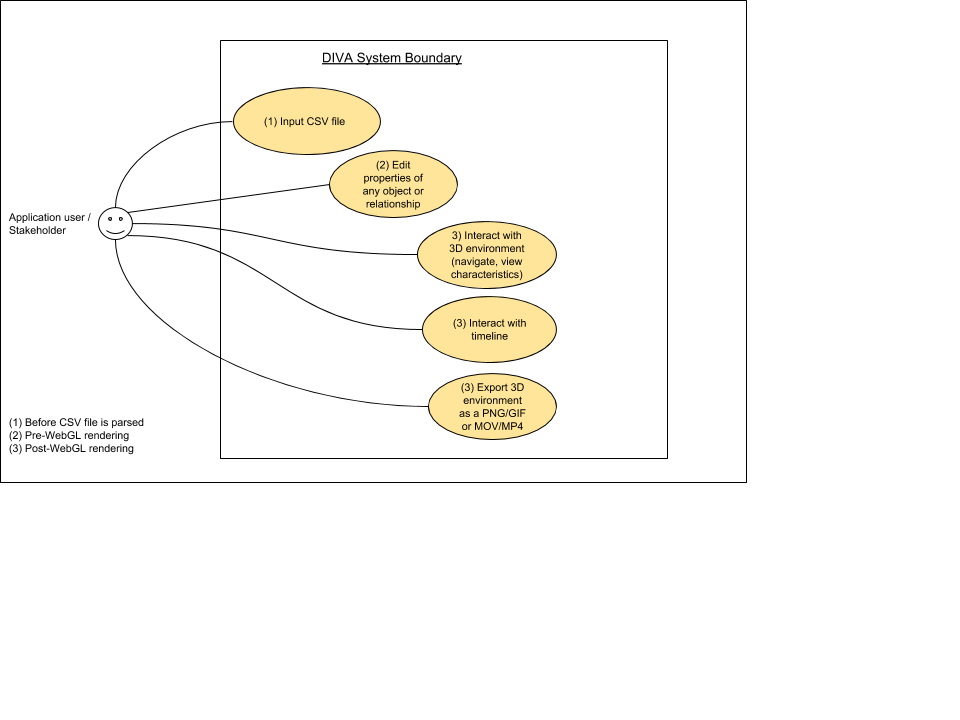
\includegraphics[width=\linewidth]{UML_1.png}
            \end{figure}
            \vspace{-4cm}
            
    %\subsection{Composition Viewpoint}
    %\subsection{Logical Viewpoint}
    %\subsection{Dependency Viewpoint}
    %\subsection{Information Viewpoint}
    %\subsection{Patterns Use Viewpoint}
    
    \subsection{Interface Viewpoint}
        The interfaces described in the SRS include only externally facing elements, of which the end user would interact with. The interfaces not mentioned in the SRS include internal components only, which are only available to modules that do not communicate directly with the end user. These include:
        \begin{itemize}
            \item The interface used to send parsed data from the CSV file input module to the component which creates objects and relationships.
            \item The interface used to rebuild objects and relationships after their characteristics are edited by the user.
            \item The interface used to communicate object and relationship data to the WebGL platform for rendering.
            \item The interface used to convert screen shots of the rendered 3D environment to an image, animation, or video file.
        \end{itemize}
        
    \subsection{Structure Viewpoint}
        The design of the DIVA web application will be composed of several different modules, all of which are independent yet rely on the output of one another to perform their function. By creating a modular setting such as this, each component will act in it's own local context, giving each module it's own unique structure and configuration. There are several benefits to developing the DIVA web application in this way, including an improved distribution of work between the development team and easier manipulation of the application's architecture.
        
    \subsection{Interaction Viewpoint}
    The DIVA web application's modules are designed to interact with two general entities: the end user, and other modules within the application. Interaction by the user is based off of the following scenarios: adding or editing the data to be rendered into a 3D environment, interacting with the 3D environment and timeline, and downloading the 3D environment for offline display. These interactions by the user will involve the modules defined in section 5.2.3 (\textit{Example Languages}). The interactions between the internally facing modules will be mostly singular and limited - meaning for every run-through of the application, each module should only be executed once. The only exception for this would be the pre-rendering module which edits parsed CSV values before WebGL rendering, which can take place an unlimited number of times before the user decides to render the values. 
    
%    \subsection{State Dynamics Viewpoint}
%    \subsection{Algorithm Viewpoint}
%    \subsection{Resource Viewpoint}

\newpage
\section*{Annex A (informative) Bibliography}
\begingroup
\renewcommand{\section}[2]{}
\bibliographystyle{IEEEtran}
\bibliography{ref.bib}
\endgroup

%\section*{Annex B (informative) Conforming Design Language Description}
%\section*{Annex C (informative) Templates For an SDD}

\end{document}